\documentclass{sysuthesis}

%%
% 论文相关信息
% 本文档中前缀"c-"代表中文版字段, 前缀"e-"代表英文版字段
% modifyer: 黄俊杰(huangjj27, 349373001dc@gmail.com)
% update date: 2017-04-13
%%

% 标题
% 论文题目应以简短、明确的词语恰当概括整个论文的核心内容,避免使用不常见的缩略词、缩写字。读者通过标题可大致了解毕业设计(论文)的内容、专业的特点和科学的范畴。中文题目一般不宜超过 24 个字,必要时可增加副标题。外文题目一般不宜超过 12 个实词

% 封面标题。由于技术所限,封面题目过长的划分交由用户您进行定夺
% 这也能让您的论文封面看起来更有美感
\covertitlefirst{中山大学}
\covertitlesecond{本科毕业论文非正式模版}

% Author:   Souler Ou
% 修改者:    欧一锋
% Date:     3/30/2018
% Mail:     ou@souler.cc
%如果英文标题过长可以使用此两项作为表三(答辩记录表)的标题。
\etitlefirst{Unofficial \Latex\ Template}
\etitlesecond{for SYSU Graduation Thesis}

% 另外一种封面的论文题目. 换行使用换行符("\\")
%\title{
%    中山大学 \\
%    本科毕业论文非正式模版
%}

% 中文标题
\ctitle{自动驾驶场景下基于深度学习方法的三维物体追踪}
\etitle{Deep Learning Based Method for 3-D Object Tracking in Automatic Drive Scene}

% 解决英文摘要页标题过长问题 (Issue 49&63)
% 当\etitle的长度超过页边距时,请使用下面的命令自行断行
% 此操作只影响英文摘要页的标题,不影响页眉的标题
% 如果不需要断行,将\eabstracttitlesecond{ }留空即可
\eabstracttitlefirst{Unofficial \LaTeX\ Template} 
\eabstracttitlesecond{for SYSU Graduation Thesis}

% 作者详细信息
\author{韩硕轩}
\cauthor{韩\ 硕\ 轩}    % 封面作者
\eauthor{Han Shuoxuan}
\studentid{15352102}
\cschool{数据科学与计算机学院}

\cmajor{软件工程(移动信息工程)}
\emajor{Software Engineering}

% 指导老师
\cmentor{黄凯\ 教授}
\ementor{Prof. Huang Kai}

     % 论文相关信息
%%
% 开题报告
% modifier: 黄俊杰(huangjj27, 349373001dc@gmail.com)
% update date: 2017-05-14

\usepackage{indentfirst}

% 选题目的
\objective{
\indent 自动驾驶是近年来的研究热点之一,拥有广阔的应用场景和强大的市场支持。自动驾驶的核心是环境感知,即让一辆车较为精确地感知周围环境。在驾驶环境中,车辆对行人的识别,对障碍物的检测和对路径的规划等都需要它能很好地理解环境。本项目基于激光雷达采集的三维点云数据集,采用深度学习的方法,目的是改善现有的物体追踪效果,从而为后续的决策提供可靠基础。
}

% 思路
\methodology{
\indent 激光雷达是自动驾驶领域应用最为广泛的传感器之一,它能采集到高分辨率的三位点云数据。深度学习为计算机视觉提供了重要的研究手段,它能在看似混杂的数据中提取出特征供机器来学习。因此本项目基于激光雷达采集到的三维点云数据集,并采用深度学习方法进行研究。
}
% 研究方法/程序/步骤
\researchProcedure{
\indent 本项目以一种物体检测效果显著的开源深度学习框架为基础,融合另一种物体追踪框架模型中的部分方法,进一步修改成为现在提出的Correlated-Voxelnet。
}

% 相关支持条件
\supportment{
实验室服务器:四路Tesla M40 GPU;
\newline 天河二号超算节点:tianhe2-G集群。
}

% 进度安排
\schedule{
第一阶段:2018年11月 - 2018年12月
\newline 论文调研,对目前已经被提出的研究方法建立全面的了解。
\newline 第二阶段:2019年1月 - 2019年2月
\newline 算法实现阶段。运用深度学习框架,结合多帧融合数据实现三维场景下的物体追踪。
\newline 第三阶段:2019年3月
\newline 代码调整和优化,以及论文写作。针对结果进行代码调整和参数优化,使得系统准确性和可靠性达到最优。同时撰写和修改论文。
}

% 指导老师意见
\proposalInstructions{

}

   % 开题报告内容
%%
% 摘要信息
% 本文档中前缀"c-"代表中文版字段, 前缀"e-"代表英文版字段
% 摘要内容应概括地反映出本论文的主要内容,主要说明本论文的研究目的、内容、方法、成果和结论。要突出本论文的创造性成果或新见解,不要与引言相 混淆。语言力求精练、准确,以 300—500 字为宜。
% 在摘要的下方另起一行,注明本文的关键词(3—5 个)。关键词是供检索用的主题词条,应采用能覆盖论文主要内容的通用技术词条(参照相应的技术术语 标准)。按词条的外延层次排列(外延大的排在前面)。摘要与关键词应在同一页。
% modifier: 黄俊杰(huangjj27, 349373001dc@gmail.com)
% update date: 2017-04-15
%%

\cabstract{
自动驾驶技术是近年来的一个研究热点。如何让车辆精确地感知周围环境是自动驾驶场景中的一个难题,而在传感器采集的一段连续数据中追踪道路上别的车辆就是环境感知的一部分。本文提出了一种融合两种开源框架的方法。该算法不仅对于每一帧数据都做独立的检测,还利用帧与帧之间场景变化较平稳的特点提取它们的相似性,从而优化检测结果,并达到更优的追踪效果。
}
\ckeywords{自动驾驶;激光雷达;深度学习;计算机视觉;点云;物体追踪}

\eabstract{
Automous driving technology is a research hotspot in recent years. Making a vehicle accurately perceive the surrounding environment is a difficult problem in automatic driving scenarios, and tracking other vehicles on the road from continuous data collected by sensors is a part of this. This paper proposes a fused method of two open source frameworks. It not only detects each frame data independently, but also extracts their similarities between adjacent frames, since the features of change stably, thus to optimize the detection results and achieve better tracking effect.
}
\ekeywords{Autonomous Driving, LiDAR(Light Detection And Ranging), Deep Learning, Computer Vision, Point Cloud, Object Tracking}

     % 摘要内容
%%
% 成绩评定记录表
% modifier: 黄俊杰(huangjj27, 349373001dc@gmail.com)
% update date: 2017-05-17

\gradingComment{
  某某同学针对什么问题研究了什么算法/实现了什么系统/针对这个系统做了什么测试,本文选题合理,实验结果表明技术路线……论文写作规范,引用文献充分,符合中山大学本科论文的规范,是篇优秀/良好/中等/合格的论文。
}
    % 成绩评定记录表评语
%%
% 四次进度报告相关信息

% Author:   Souler Ou
% 修改者:    欧一锋
% Date:     3/30/2018
% Mail:     ou@souler.cc

% 第一次进度报告
\firstsummary{
	\begin{adjustwidth}{2em}{2em}
		在这一阶段,XXX工作基本完成,主要在如下几个方面:
		\begin{enumerate}
			\item 完成了第一项。
			\item 完成了第二项
			\item 完成了第三项。 
		\end{enumerate}
	\end{adjustwidth}
}
% 第2次进度报告
\secondsummary{
	\begin{adjustwidth}{2em}{2em}
		...
	\end{adjustwidth}
}
% 第3次进度报告
\thirdsummary{
	\begin{adjustwidth}{2em}{2em}
		...
	\end{adjustwidth}
}
% 第4次进度报告
\fourthsummary{
	\begin{adjustwidth}{2em}{2em}
		...
	\end{adjustwidth}
}
% 第1次老师评价
\firstcomment{
	\begin{adjustwidth}{2em}{2em}
		论文完成情况良好。
	\end{adjustwidth}
}
% 第2次老师评价
\secondcomment{
	\begin{adjustwidth}{2em}{2em}
		...
	\end{adjustwidth}
}
% 第3次老师评价
\thirdcomment{
	\begin{adjustwidth}{2em}{2em}
		...
	\end{adjustwidth}
}
% 第4次老师评价
\fourthcomment{
	\begin{adjustwidth}{2em}{2em}
		...
	\end{adjustwidth}
}
% 老师总评价
\finalcomment{
	\begin{adjustwidth}{2em}{2em}
		...
	\end{adjustwidth}
}   % 过程检查报告数据
\begin{document}
    % 论文前置部分
    \frontmatter
        \pagenumbering{Roman}
        \maketitle    % 封面
        \makeProposal% 开题报告
        \makeProgressCheck  % 过程检查记录表
        \makeDefenseRecord  % 答辩情况等级表
        \makedisclaim       % 学术诚信声明
        \makeabstract       % 中英文摘要
        \maketableofcontents        % 目录
        \makelistoffiguretable

    % 论文主体部分
    \mainmatter
        % 引言

        % 正文
        %%
% 引言或背景
% 引言是论文正文的开端,应包括毕业论文选题的背景、目的和意义;对国内外研究现状和相关领域中已有的研究成果的简要评述;介绍本项研究工作研究设想、研究方法或实验设计、理论依据或实验基础;涉及范围和预期结果等。要求言简意赅,注意不要与摘要雷同或成为摘要的注解。
% modifier: 黄俊杰(huangjj27, 349373001dc@gmail.com)
% update date: 2017-04-15
%%

\chapter{引言}
\label{cha:introduction}
\section{选题背景与意义}
\label{sec:background}
让机器节省甚至替代人力一直是科技发展的大方向。自动驾驶汽车,一种通过传感器和电脑实现无人驾驶的智能汽车,则是近些年来越来越受到关注的一个研究热点。如果自动驾驶技术能在生活中得到广泛应用,那么人们的生活质量将大幅提高。举两个很贴近校园生活的例子:很多学校都有校内接送学生的电动车,它的时间和线路相对固定,驾驶巴士的司机常年做着重复劳动,十分枯燥;很多同学喜欢叫外卖,因此无数的递送员每天奔波于商家和宿舍之间,还经常因为无法按时送达被投诉。但假如能应用成熟的自动驾驶技术,这样的情况将得到极大改善。不仅如此,在国家快速现代化发展的大环境下,自动驾驶还可以缓解城市交通拥堵、交通事故发生频繁等问题。所以,自动驾驶技术的发展对于国家和社会具有重要意义。

虽然自动驾驶技术距离广泛应用还有一定的距离,但相关研究工作已经在国内外各大企业和高校如火如荼地展开。为了方便区分和定义自动驾驶的程度,国际自动机工程师学会(SAE)提出了一套分级标准,将自动驾驶分为了L0到L5六个等级(如图1-1)。其中L0和L1实现自动化的程度非常低,需要人类驾驶员执行几乎所有操作。而到了L2,控制方向和加减速的操作就可以由汽车自己完成,驾驶员需要监视,准备随时接管以完成其他操作。到了L3,驾驶员已经可以解放手脚了,但仍需保持注意力集中。而L4和L5则已经无需驾驶员的控制,完全由汽车自己掌握全部操作,只是L4对道路环境有特殊要求。目前很多汽车制造商的技术都达到了L2级别,比如Tesla的Autopilot 2.0和Volvo的S60。谷歌测试中的无人车处在L3的阶段。而硅谷一家2016年成立的公司Nuro声称他们的配送车可以不用人类驾驶员,也就是至少达到了L4的水平。
\begin{figure}[h]
	\centering
	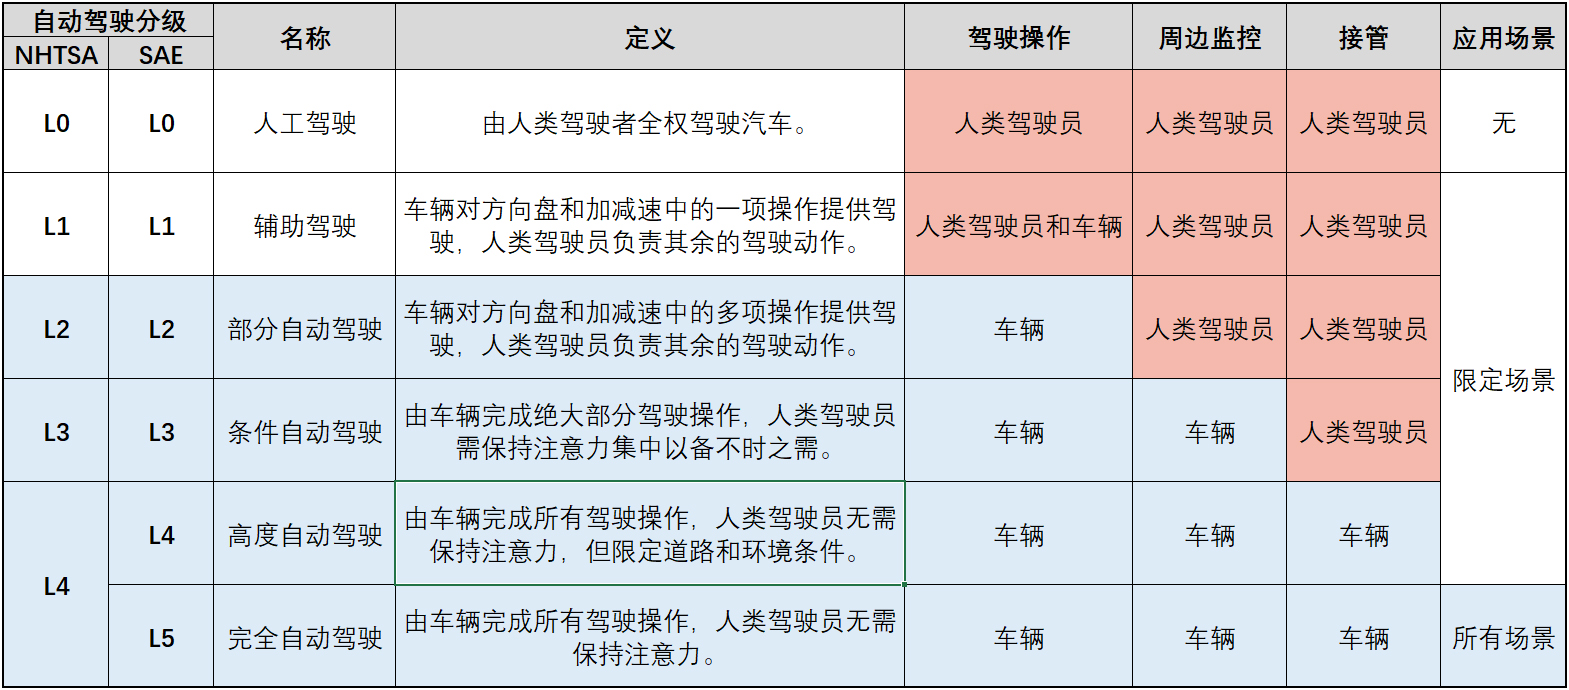
\includegraphics[width=0.5\textwidth]{image/自动驾驶等级.jpg}
	\caption{SAE提出的自动驾驶等级}
 	\label{fig:1-1}
\end{figure}


自动驾驶中的一大难点是环境感知,即采用什么样的传感器,以及如何将传感器采集的环境数据转化为机器可以理解的数据。对于这个问题,不同的实验室有不同的解决方案。Tesla使用的是视觉摄像头。由于视觉摄像头成本低廉,且图像检测算法已经较为成熟,所以纯视觉方法应用更为广泛。但是视觉摄像头,无论单目还是多目,都很难捕捉到准确的三维信息,因为它们很容易受到环境中光线变化、障碍物遮挡等的影响。谷歌旗下的Waymo和百度的Apollo则更多使用激光雷达。激光雷达的优点在于稳定性高,对空间感知能力强。然而它的成本高昂,且基于它采集的三维数据的算法复杂度较高,所以如何将其很好地应用还有待进一步研究。

\section{问题描述}
\label{sec:problem_description}
自动驾驶场景下的三维物体追踪,主要目标是:基于激光雷达在实际道路场景采集的三维点云数据(kitti数据集),追踪其中的多辆汽车,用三维的立方体框将它们在点云中准确地标识出来。由于数据集由一段一段连续的点云流构成,帧与帧之间不存在剧烈的变化,所以相邻帧之间的特征图具有一定的共性。如果我们能对点云流的这一特点加以利用,则将进一步提升最终的效果。

\section{本文的工作}
\label{sec:key_work}
针对上文提到的主要目标和优化方向,本项目融合了两种开源框架。其中,Voxelnet中的特征学习(feature learning)是框架的主要部分,而Detect to Track(下文简称D&T)中的相关层(correlation layer)则可以很好地发掘相邻帧之间特征的相似性。为了适配相关层的输入和输出,我们对点云读取方式和损失函数计算方式也做出了相应的调整。总结本文具体的创新和贡献如下:
\begin{itemize}
	\item 采用合并相邻两帧的方式读取点云数据。
	\item 采用Voxelnet学习特征,同时用D&T的相关层发掘相邻帧的相似性。
	\item 在损失函数中加入相关损失(correlation loss)。
\end{itemize}

\section{论文结构与章节安排}
\label{sec:arrangement}
本文共分为五章,各章节内容安排如下:

第一章引言。

第二章综述。

第三章方法、原理和框架。

第四章实验和结果。

第五章总结与展望。


        \newclearpage
        \chapter{综述}
\label{cha:review}
本章综述,将对整个项目基于的数据集和采用的方法做一个简要概述。首先是激光雷达以及国外研究团队用它采集到的kitti数据集:整个框架的训练、验证和测试都在该数据集上完成。由于本项目只采用了激光雷达采用的三维点云数据集,所以纯RGB图像方法或者图像和点云结合的方法将不被提到。接下来是分别对点云物体检测和视频流物体追踪两个领域主要方法的介绍。本项目融合的Voxelnet和D&T就分别来自这两个领域。

\section{激光雷达}
\label{LiDAR}

\section{kitti数据集}
\label{sec:kitti}

\section{点云物体检测}
\label{sec:Detection_in_Point_Cloud}

\section{视频流物体追踪}
\label{sec:Tracking_in_Video}




        \newclearpage
        \chapter{研究方法}
\label{cha:method}

        \newclearpage
        %% chapter 4 dataset, network structure, experiment and result
\chapter{实验与结果}
\label{cha:experiment}


        \newclearpage
        %%
% 结论
% 结论是毕业论文的总结,是整篇论文的归宿,应精炼、准确、完整。结论应着重阐述自己的创造性成果及其在本研究领域中的意义、作用,还可进一步提出需要讨论的问题和建议。
% modifyer: 黄俊杰(huangjj27, 349373001dc@gmail.com)
% update date: 2017-04-13
%%

\chapter{总结与展望}
\section{工作总结}
\indent 本文所述框架是基于两种效果显著的三维物体检测与追踪开源框架改进而来。
\indent 然而,在追踪取得较高精确度的同时,该框架的速度还有待提升。目前的追踪速度只有约2秒每帧,尚不能达到自动驾驶的要求。
\section{研究展望}
\indent 随着硬件设备的性能不断提高,伴随5G时代的到来,自动驾驶汽车的各个部件之间的通讯将更加稳定高效,而日渐成熟的三维物体检测与追踪技术也将为人们带来更安全和舒适的自动驾驶体验。
        \newclearpage
        % 结语

    % 附录部分
    \backmatter
        % 参考文献. 因不需要纳入章节目录, 故放入附录部分
        % 实际上参考文献是属于论文主体部分
        \makereferences

        %%
% 致谢
% 谢辞应以简短的文字对课题研究与论文撰写过程中曾直接给予帮助的人员(例如指导教师、答疑教师及其他人员)表示对自己的谢意,这不仅是一种礼貌,也是对他人劳动的尊重,是治学者应当遵循的学术规范。内容限一页。
% modifier: 黄俊杰
% update date: 2017-04-15
%%

\chapter{致谢}

	四年时间转眼即逝,青涩而美好的本科生活快告一段落了。回首这段时间,我不仅学习到了很多知识和技能,而且提高了分析和解决问题的能力与养成了一定的科学素养。虽然走过了一些弯路,但更加坚定我后来选择学术研究的道路,实在是获益良多。这一切与老师的教诲和同学们的帮助是分不开的,在此对他们表达诚挚的谢意。

	首先要感谢的是我的指导老师林倞教授。我作为一名本科生,缺少学术研究经验,不能很好地弄清所研究问题的重点、难点和热点,也很难分析自己的工作所能够达到的层次。林老师对整个研究领域有很好的理解,以其渊博的知识和敏锐的洞察力给了我非常有帮助的方向性指导。他严谨的治学态度与辛勤的工作方式也是我学习的榜样,在此向林老师致以崇高的敬意和衷心的感谢。

	最后我要感谢我的家人,正是他们的无私的奉献和支持,我才有了不断拼搏的信息的勇气,才能取得现在的成果。

\vskip 108pt
\begin{flushright}
	陈冠英\makebox[1cm]{} \\
\today
\end{flushright}

    % 致谢
        \newclearpage
        % 附录
    \appendix
        \chapter{补充更多细节}

\begin{figure}[h!]
\centering
		\makebox[0.16\textwidth]{\scriptsize 图像}
		\makebox[0.16\textwidth]{\scriptsize 真值}
		\makebox[0.16\textwidth]{\scriptsize Grid-5LSTM1}
		\makebox[0.16\textwidth]{\scriptsize Grid-5LSTM3}
		\makebox[0.16\textwidth]{\scriptsize Grid-5LSTM5} \\
		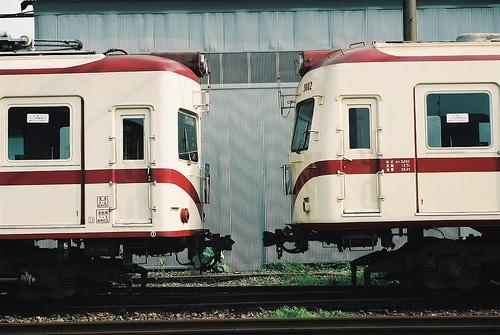
\includegraphics[width=0.16\textwidth]{image/appendix1/2007_000042.jpg}
		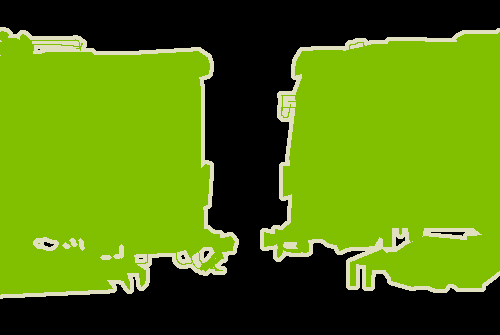
\includegraphics[width=0.16\textwidth]{image/appendix1/2007_000042.png}
		
\includegraphics[width=0.16\textwidth]{image/appendix1/1/2007_000042.png} 
		
\includegraphics[width=0.16\textwidth]{image/appendix1/3/2007_000042.png}
		
\includegraphics[width=0.16\textwidth]{image/appendix1/5/2007_000042.png} \\

		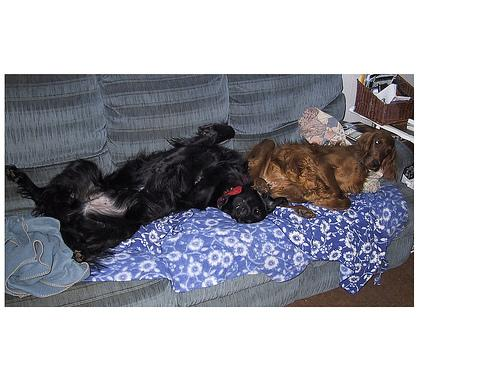
\includegraphics[width=0.16\textwidth]{image/appendix1/2011_003256.jpg}
		
\includegraphics[width=0.16\textwidth]{image/appendix1/2011_003256.png}
		
\includegraphics[width=0.16\textwidth]{image/appendix1/1/2011_003256.png} 
		
\includegraphics[width=0.16\textwidth]{image/appendix1/3/2011_003256.png}
		
\includegraphics[width=0.16\textwidth]{image/appendix1/5/2011_003256.png} \\
		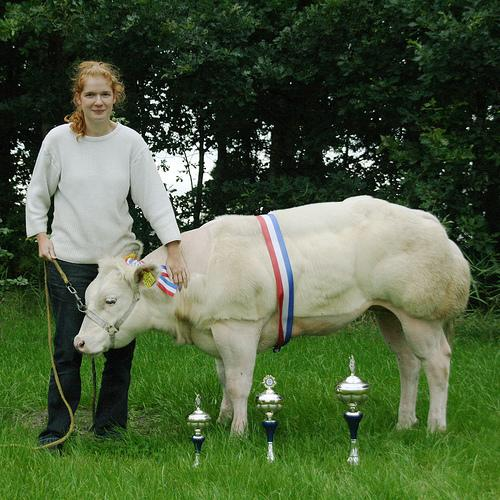
\includegraphics[width=0.16\textwidth]{image/appendix1/2011_001159.jpg}
		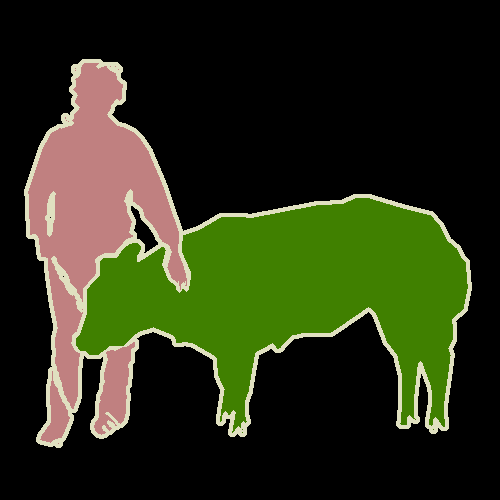
\includegraphics[width=0.16\textwidth]{image/appendix1/2011_001159.png}
		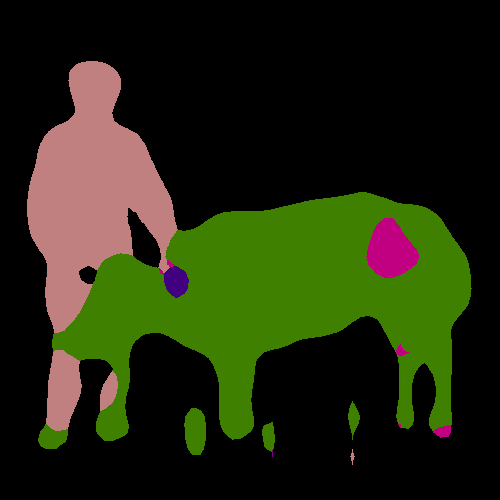
\includegraphics[width=0.16\textwidth]{image/appendix1/1/2011_001159.png} 
		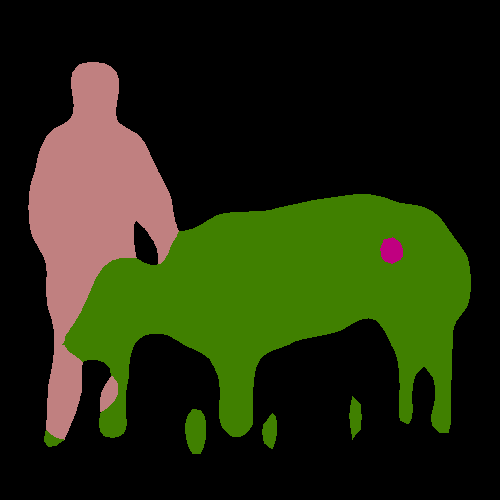
\includegraphics[width=0.16\textwidth]{image/appendix1/3/2011_001159.png}
		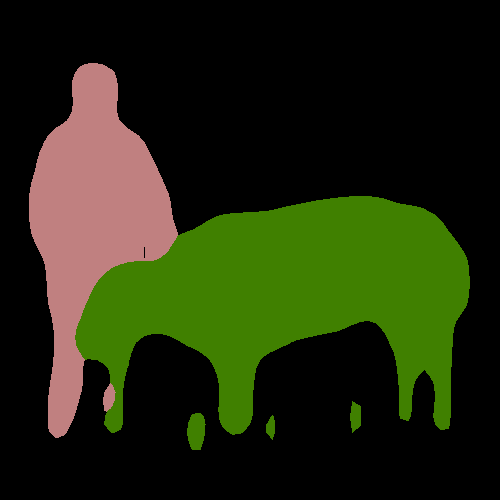
\includegraphics[width=0.16\textwidth]{image/appendix1/5/2011_001159.png} \\
		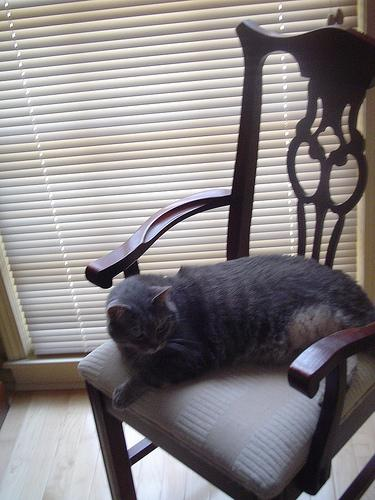
\includegraphics[width=0.16\textwidth]{image/appendix1/2011_000813.jpg}
		
\includegraphics[width=0.16\textwidth]{image/appendix1/2011_000813.png}
		
\includegraphics[width=0.16\textwidth]{image/appendix1/1/2011_000813.png} 
		
\includegraphics[width=0.16\textwidth]{image/appendix1/3/2011_000813.png}
		
\includegraphics[width=0.16\textwidth]{image/appendix1/5/2011_000813.png} \\
		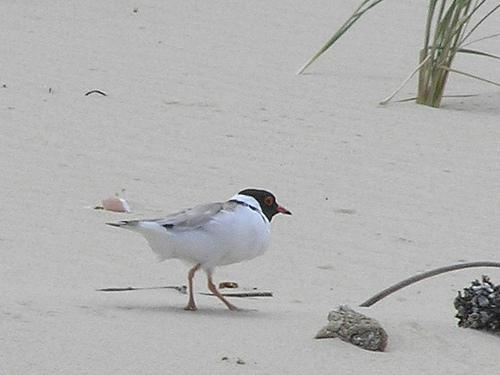
\includegraphics[width=0.16\textwidth]{image/appendix1/2011_003145.jpg}
		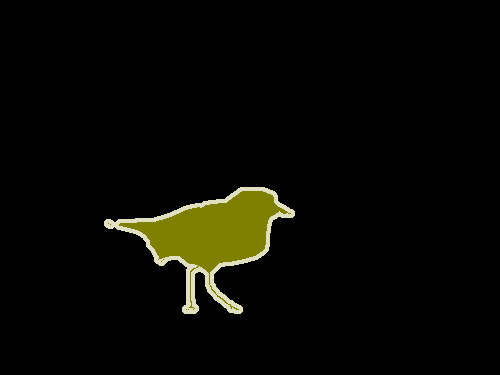
\includegraphics[width=0.16\textwidth]{image/appendix1/2011_003145.png}
		
\includegraphics[width=0.16\textwidth]{image/appendix1/1/2011_003145.png} 
		
\includegraphics[width=0.16\textwidth]{image/appendix1/3/2011_003145.png}
		
\includegraphics[width=0.16\textwidth]{image/appendix1/5/2011_003145.png} \\
		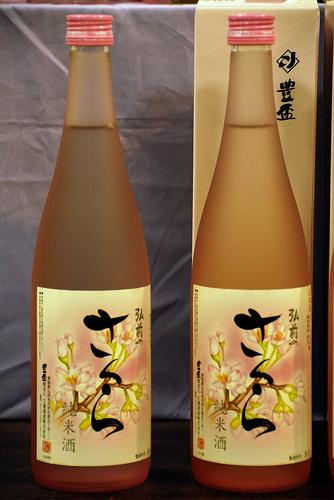
\includegraphics[width=0.16\textwidth]{image/appendix1/2009_004579.jpg}
		
\includegraphics[width=0.16\textwidth]{image/appendix1/2009_004579.png}
		
\includegraphics[width=0.16\textwidth]{image/appendix1/1/2009_004579.png} 
		
\includegraphics[width=0.16\textwidth]{image/appendix1/3/2009_004579.png}
		
\includegraphics[width=0.16\textwidth]{image/appendix1/5/2009_004579.png} \\
\color[rgb]{0.9,0.9,0.9}\bfseries
\begin{tabular}{*{7}{>{\centering\arraybackslash}p{0.10\textwidth}}}
	\hline
	\cellcolor[rgb]{0,0,0}  背景&\cellcolor[rgb]{0.5020,0,0} 飞机 &\cellcolor[rgb]{0,0.5020,0} 自行车 &\cellcolor[rgb]{0.5020,0.5020,0} 鸟 &\cellcolor[rgb]{0,0,0.5020} 船   &\cellcolor[rgb]{0.5020,0,0.5020} 瓶子 &\cellcolor[rgb]{0,0.5020,0.5020} 大巴
	\\
	\hline
	\cellcolor[rgb]{0.5020,0.5020,0.5020} 汽车 & \cellcolor[rgb]{0.2510,0,0} 猫 &\cellcolor[rgb]{0.7529,0,0} 椅子 &\cellcolor[rgb]{0.2510,0.5020,0} 牛 &\cellcolor[rgb]{0.7529,0.5020,0} 桌子 &\cellcolor[rgb]{0.2510,0,0.5020} 狗 &\cellcolor[rgb]{0.7529,0,0.5020} 马 \\
	\hline
	\cellcolor[rgb]{0.2510,0.5020,0.5020} 摩托车 &\cellcolor[rgb]{0.7529,0.5020,0.5020} 人   &\cellcolor[rgb]{0,0.2510,0} 盆栽   &\cellcolor[rgb]{0.5020,0.2510,0} 羊 &\cellcolor[rgb]{0,0.7529,0} 沙发 &\cellcolor[rgb]{0.5020,0.7529,0} 火车 &\cellcolor[rgb]{0,0.2510,0.5020} 电视 \\
	\hline
\end{tabular}

\caption{一个配有彩色表格的插图}
\end{figure}

\endinput

        \newclearpage
    \makeGrade      % 成绩评定记录表
\end{document}

